\mode<article>

Para describir el problema en forma completa, las 
condiciones de contorno deben ser dadas. Comencemos
por el caso más sencillo en el que se conoce el 
valor de la función incógnita en el borde del
recinto de integración, tal como se mostró en
la figura \ref{FiuguraPresentacionProblema}.

Para poder expresar estas condiciones de contorno
en nuestro modelo computacional, debemos pensar 
primero en la numeración que recibirán los nodos
de cada borde. podemos entonces tomar los
vectores de índices que los describen. Retomando
la numeración descrita en la Figura \ref{FiguraDiscretizacion}, 
podemos escribir los siguientes vectores

\begin{equation}\label{EqNumeracionBordes}
  \begin{split}
  k_A &= \Big[1,1+Nx, \dotsi ,1+(N_y -1)N_x\Big]\\
  k_B &= \Big[Nx, 2N_x,  \dotsi , N_yN_x\Big]\\
  k_C &= \Big[1,2,\dotsi,N_x]\\
  k_D &= \Big[1+(N_y-1)N_x,2+(N_y-1)N_x,\dotsi, N_x N_y]
  \end{split}
\end{equation}

Para cualquiera de los nodos cuyo índice $k$ puede
encontrarse en alguno de los vectores de la ecuación
\ref{EqNumeracionBordes}, se tiene que la ecuación 
que \emph{deben cumplir} es

\begin{equation}\label{EqEcuacionesTFija}
  T_{k \in k_A} = T_A ;  T_{k \in k_B} = T_B ; T_{k \in k_C} = T_C ; T_{k \in k_D} = T_D
\end{equation}

Estas últimas condiciones son triviales de conseguir si 
se cambian los coeficientes de las filas de la matríz
correspondientes y el vector $\vec{b}$ como se 
muestra en la Figura \label{FiguraContornoTFija}. Se
muestra que como la ecuación se ha cambiado por 
la \ref{EqEcuacionesTFija}, solo el coeficiente 
de la diagonal es distinto de cero. El resto
de los coeficientes en las columnas no diagonales
es nulo ya que a la derecha del igual los nodos
con $ k' \neq k $ aparecen solo en forma implícita 
multiplicados por cero. 

\begin{figure}
  \includeslide[width=\textwidth]{FrameContornoTFija} 
  \caption{Coeficientes de matriz para los nodos
  en cualquiera de los bordes del recinto del problema.
  \label{FiguraContornoTFija}}
\end{figure}


\mode*

\againframe<2>{FrameProblema}

\begin{frame}<presentation>[label=FrameContornoTFija]
  \frametitle{Borde a temperatura fija}

  \begin{columns}
    \column{0.5\textwidth}
    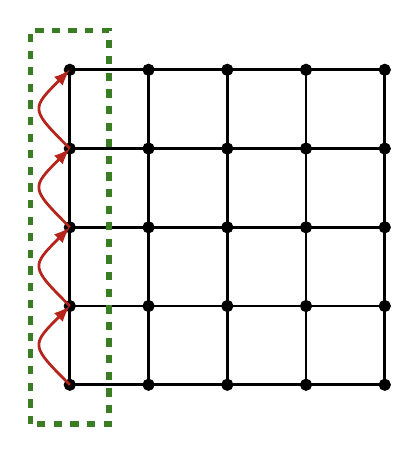
\begin{tikzpicture}
      \draw [line width=1pt] (-2,-2) grid (2,2);
      \foreach \x in {-2,-1,0,1,2}
            \foreach \y in {-2,-1,0,1,2}
	    {
	      \draw [fill=black] (\x,\y) circle (2pt);
	      };
       	
       \foreach \y in {-2,-1,0,1}
       {
	 \draw [BrickRed,->,>=latex,line width=1pt] 
	 (-2,\y) .. controls (-2.5,\y+0.5) ..  (-2,\y+1);
	 };

	 \draw [OliveGreen,dashed,line width=2pt] (-2.5,-2.5) rectangle (-1.5,2.5);
    \end{tikzpicture}
    
    \column{0.5\textwidth}

    \tikz[baseline]\node (cc) at (0,0) {$T_{k_A}=T_A$}; \hfill

    
     \mode<handout>{$k_A = \big[ 1:Nx:1+(N_y-1)N_x\big]$} \mode<beamer>{$k_A = ?$ Algun Rango ...}

    \vspace{0.5cm}

    $M_{k_A} ^{fija} = \Big[ \dotsi$ 
    \tikz[baseline] \node (diag) at (0,0) {$1$};
    $\dotsi \Big]$
    \tikz[overlay] \draw [blue, ->, >=latex ] (diag) -- ($(diag)-(0,1)$) 
    node [anchor=north,text=black] { $k_A$};

    \vspace{2cm}

    \tikz[baseline] \node (bk) [text=black,anchor=east] {$b_k = T_A$};


    \tikz[overlay] \draw [blue,->,>=latex] (cc) -| ($(bk)+(5,0)$) -- (bk); %-- (bk);

  \end{columns}

\end{frame}

\mode<all>
